\chapter{\label{annexa} Annexe A: performances des tests utilisateurs}
	\begin{figure}[h]
		\centering
		\subfloat[Étape 2: Familiarisation avec le programme]{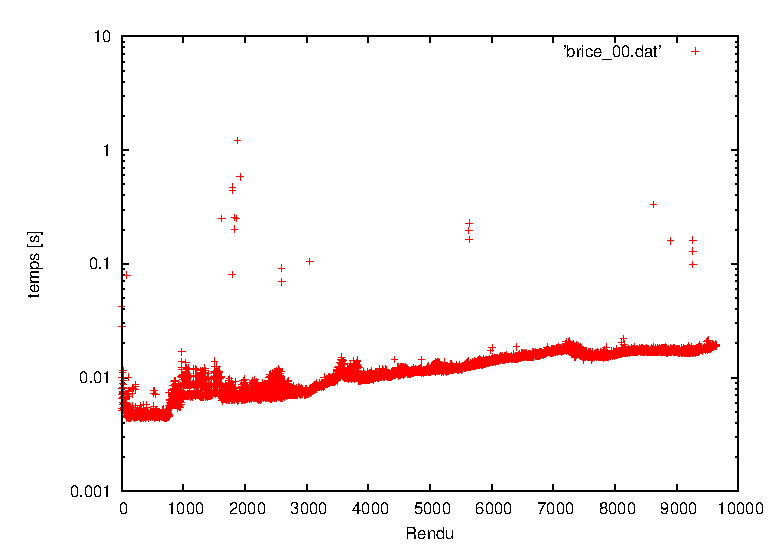
\includegraphics[width=0.6\textwidth]{images/rendertimes/brice_00.eps} }\\
		\subfloat[Étape 3: Portrait au trait]{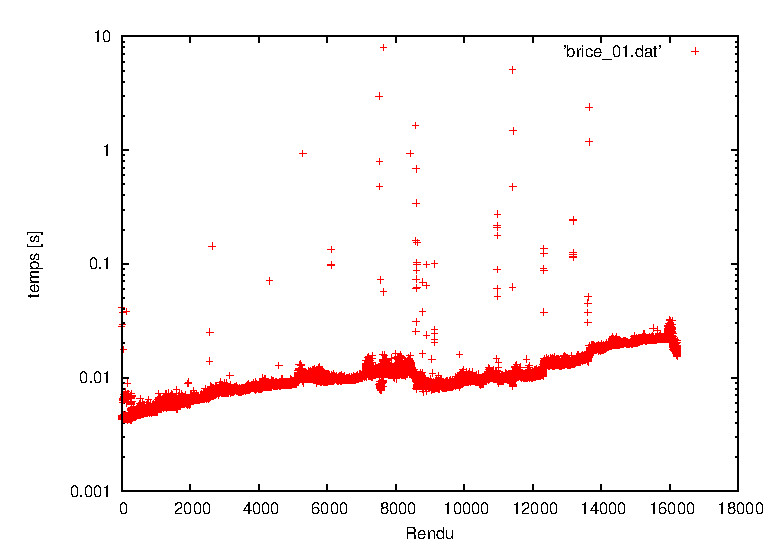
\includegraphics[width=0.6\textwidth]{images/rendertimes/brice_01.eps} }\\
		\subfloat[Étape 4: Potrait couleur]{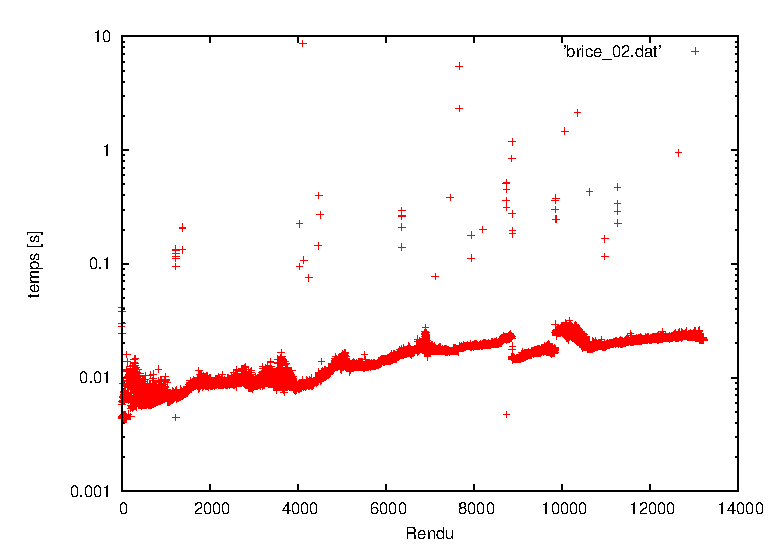
\includegraphics[width=0.6\textwidth]{images/rendertimes/brice_02.eps} }\\
		\subfloat[Étape 5: Homme avec puce sur éléphant ]{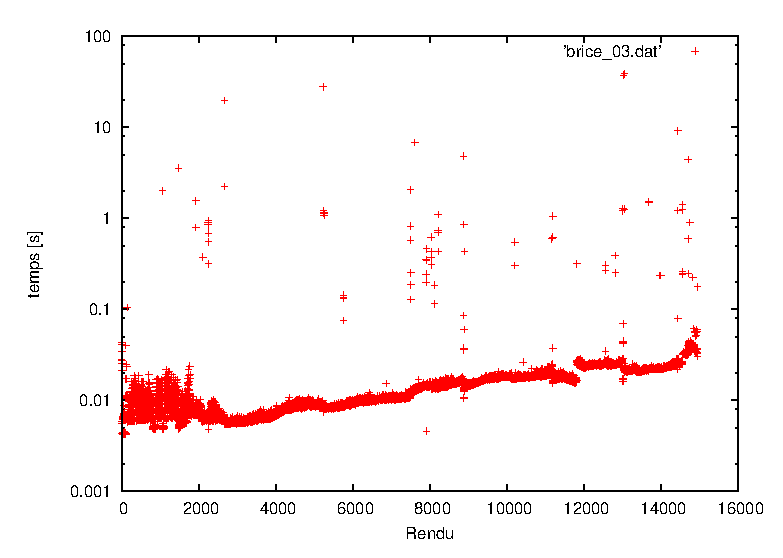
\includegraphics[width=0.6\textwidth]{images/rendertimes/brice_03.eps} }\\
		\caption{Graphe des temps de rendu des mise à jour lors des tests de \emph{Brice Vandemoortele}}
	\end{figure}
	\begin{figure}[h]
		\centering
		\subfloat[Étape 2: Familiarisation avec le programme]{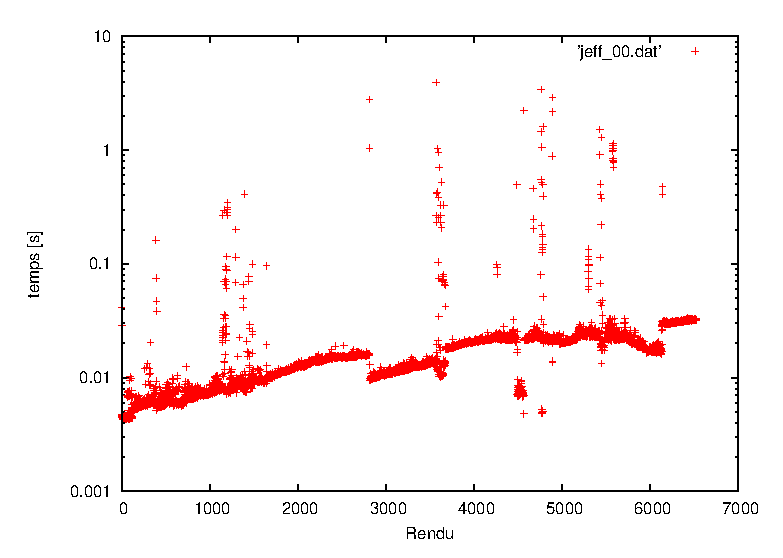
\includegraphics[width=0.6\textwidth]{images/rendertimes/jeff_00.eps} }\\
		\subfloat[Étape 3: Portrait au trait]{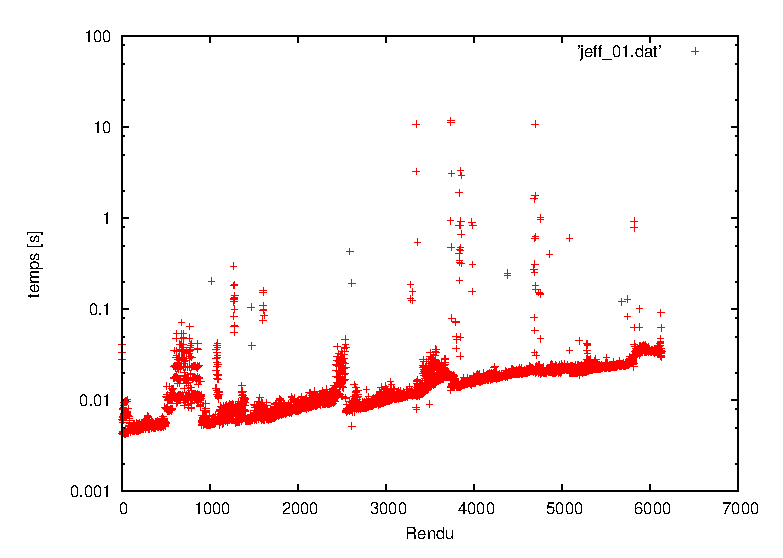
\includegraphics[width=0.6\textwidth]{images/rendertimes/jeff_01.eps} }\\
		\subfloat[Étape 4: Potrait couleur]{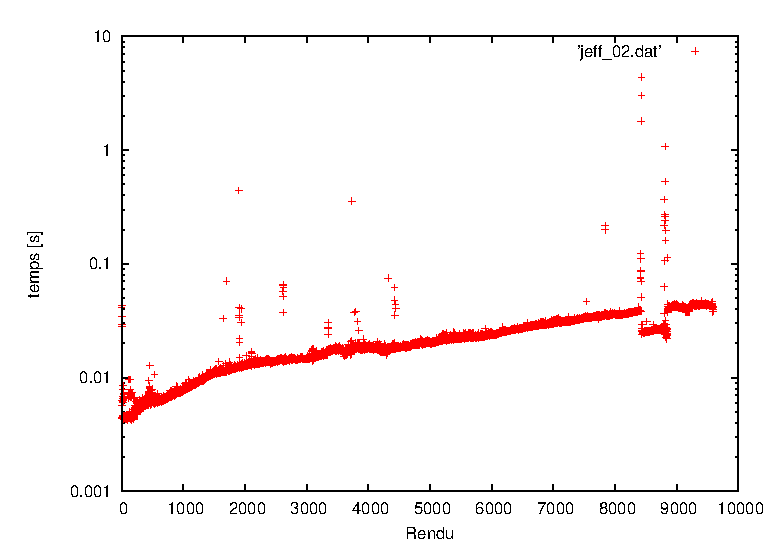
\includegraphics[width=0.6\textwidth]{images/rendertimes/jeff_02.eps} }\\
		\subfloat[Étape 5: Homme avec puce sur éléphant ]{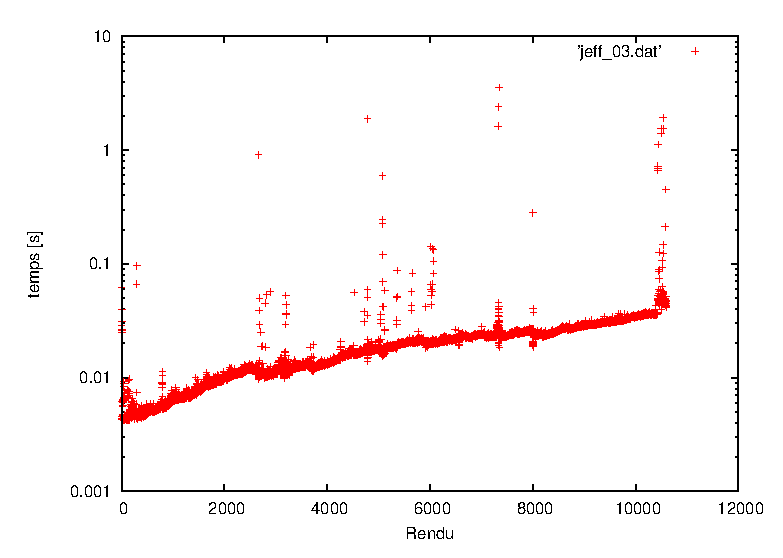
\includegraphics[width=0.6\textwidth]{images/rendertimes/jeff_03.eps} }\\
		\caption{Graphe des temps de rendu des mise à jour lors des tests de \emph{Jean-François Brogniet}}
	\end{figure}
	\begin{figure}[h]
		\centering
		\subfloat[Étape 2: Familiarisation avec le programme]{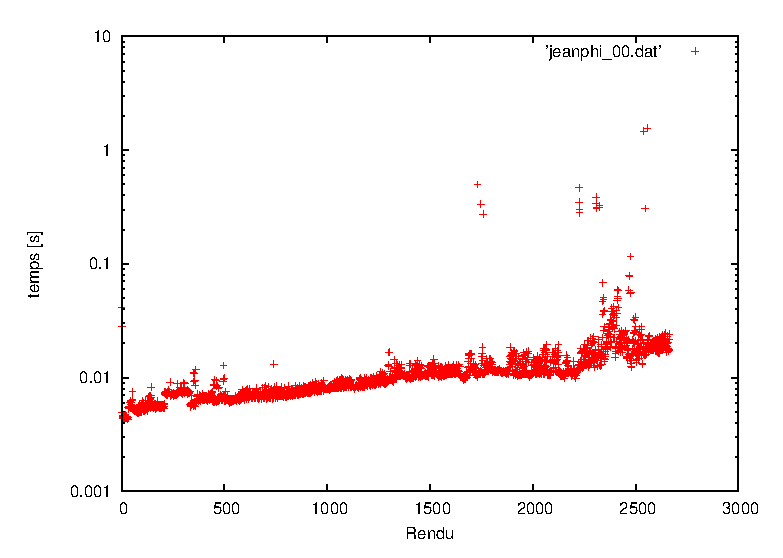
\includegraphics[width=0.6\textwidth]{images/rendertimes/jeanphi_00.eps} }\\
		\subfloat[Étape 3: Portrait au trait]{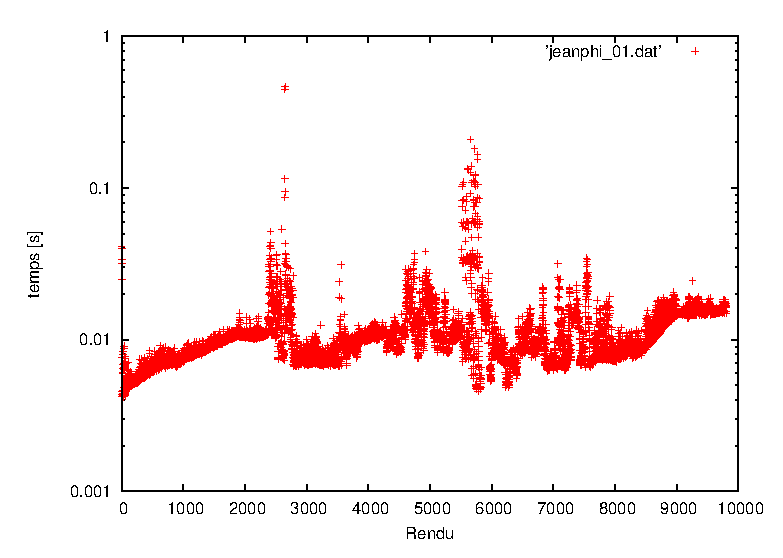
\includegraphics[width=0.6\textwidth]{images/rendertimes/jeanphi_01.eps} }\\
		\subfloat[Étape 4: Potrait couleur]{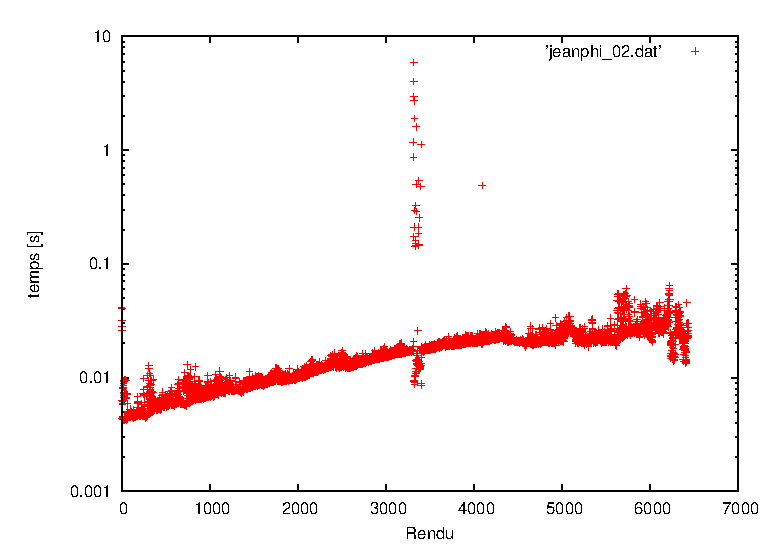
\includegraphics[width=0.6\textwidth]{images/rendertimes/jeanphi_02.eps} }\\
		\subfloat[Étape 5: Homme avec puce sur éléphant ]{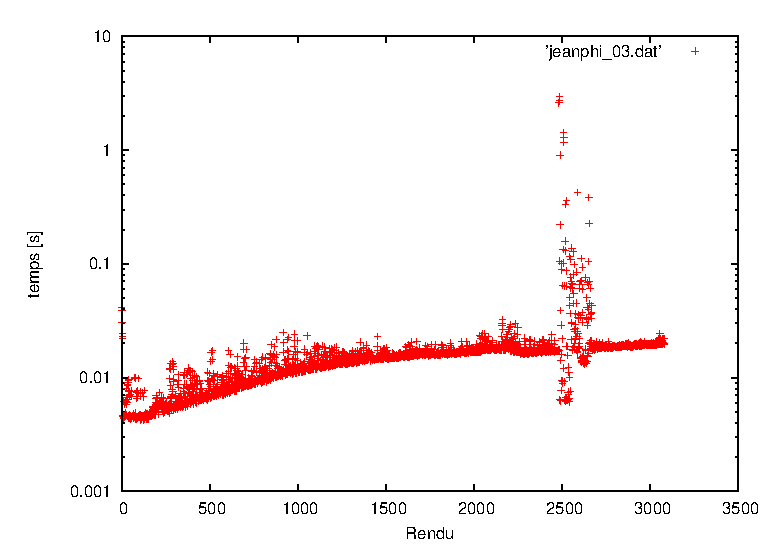
\includegraphics[width=0.6\textwidth]{images/rendertimes/jeanphi_03.eps} }\\
		\caption{Graphe des temps de rendu des mise à jour lors des tests de \emph{Jean-Philippe Servais}}
	\end{figure}
\chapter{\label{annexb} Annexe B: peintures des utilisateurs}
	\begin{figure}[h]
		\centering
		\subfloat[Étape 2: Familiarisation avec le programme]{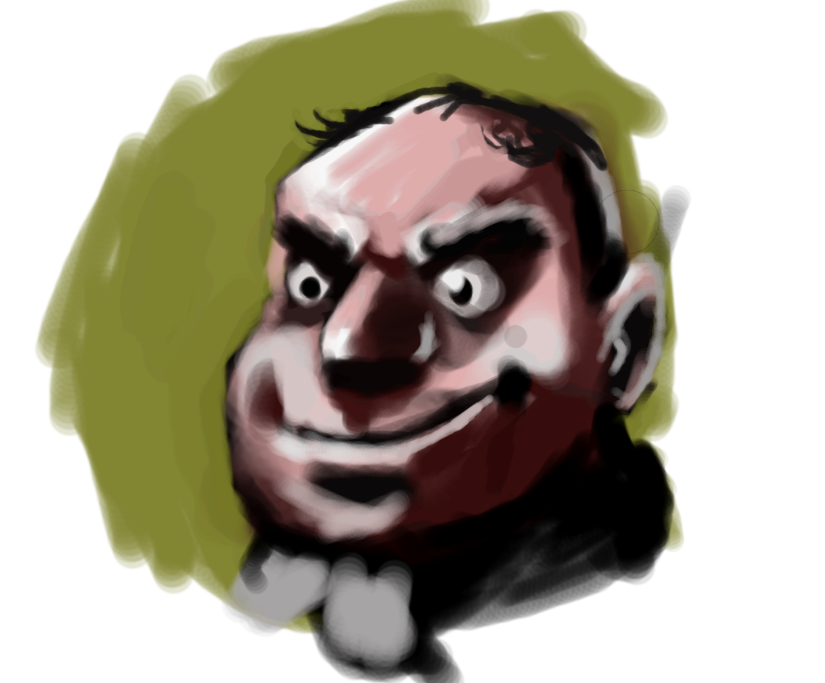
\includegraphics[width=0.5\textwidth]{images/paintings/brice0} }
		\subfloat[Étape 3: Portrait au trait]{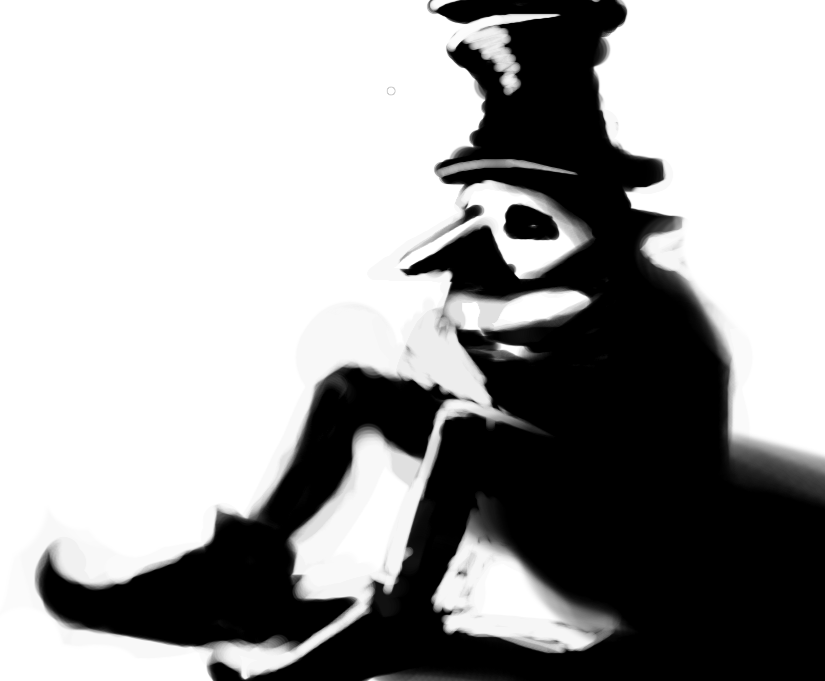
\includegraphics[width=0.5\textwidth]{images/paintings/brice1} }\\
		\subfloat[Étape 4: Potrait couleur]{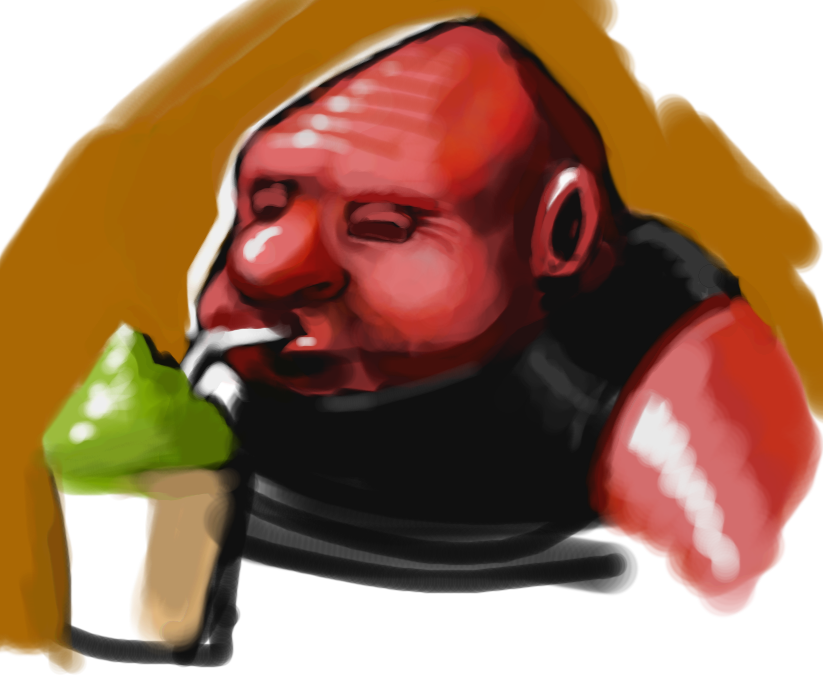
\includegraphics[width=0.5\textwidth]{images/paintings/brice2} }
		\subfloat[Étape 5: Homme avec puce sur éléphant ]{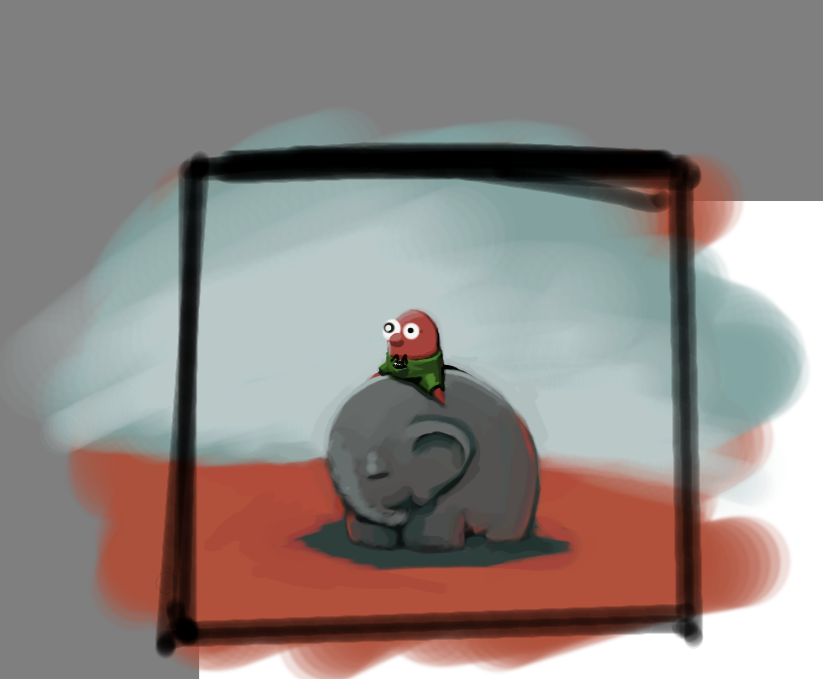
\includegraphics[width=0.5\textwidth]{images/paintings/brice3} }\\
		\subfloat[Étape 5: Homme avec puce sur éléphant : Détail]{
\includegraphics[width=0.6\textwidth]{images/paintings/brice3b} }\\
		\caption{Dessins réalisés pendant les tests par \emph{Brice Vandemoortele}}
	\end{figure}
	\begin{figure}[h]
		\centering
		\subfloat[Étape 2: Familiarisation avec le programme]{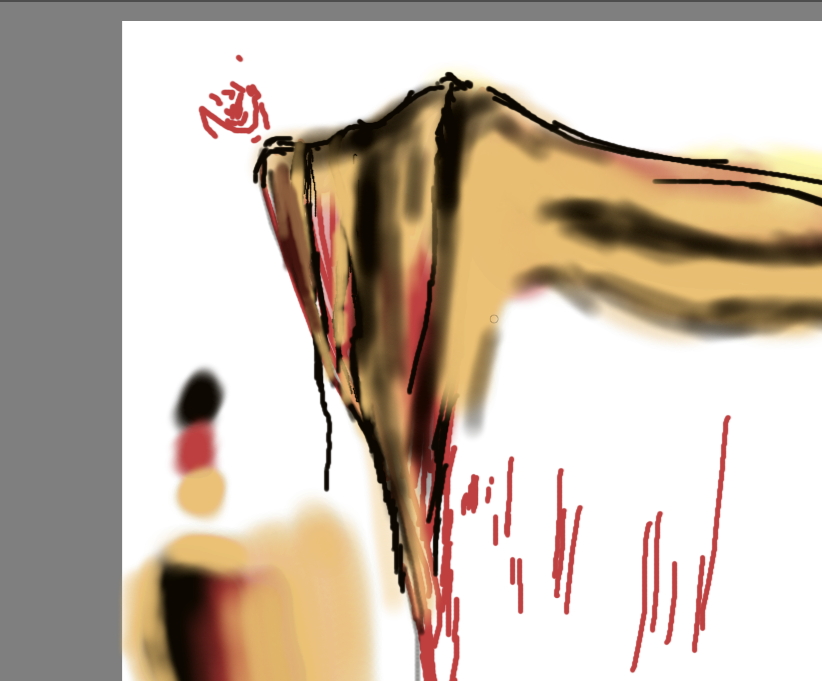
\includegraphics[width=0.5\textwidth]{images/paintings/jeff0} }
		\subfloat[Étape 3: Portrait au trait]{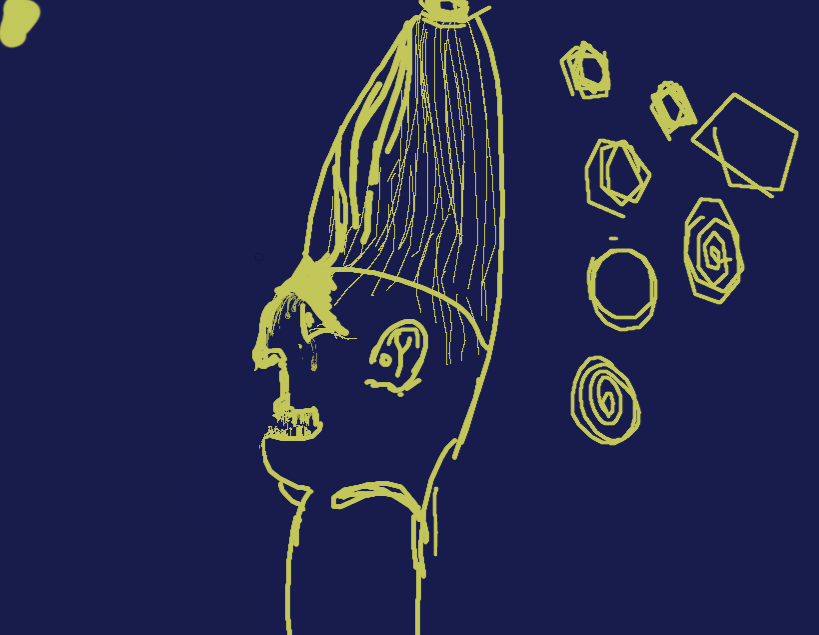
\includegraphics[width=0.5\textwidth]{images/paintings/jeff1} }\\
		\subfloat[Étape 4: Potrait couleur]{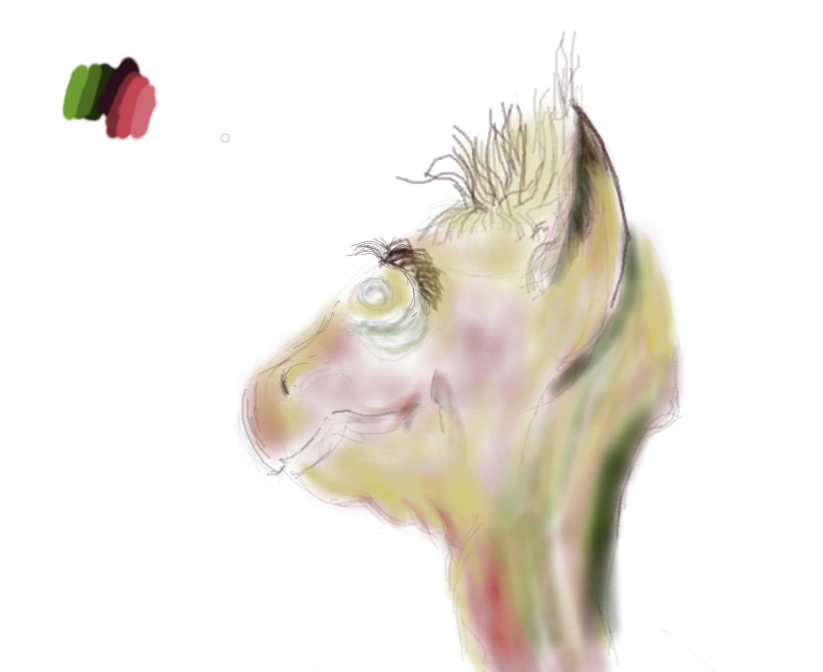
\includegraphics[width=0.5\textwidth]{images/paintings/jeff2} }
		\subfloat[Étape 5: Homme avec puce sur éléphant ]{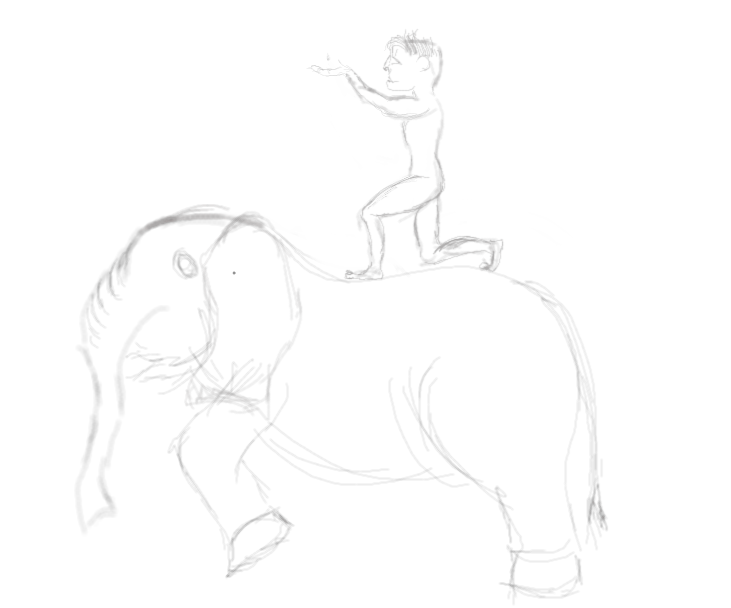
\includegraphics[width=0.5\textwidth]{images/paintings/jeff3} }\\
		\subfloat[Étape 5: Homme avec puce sur éléphant : Détail]{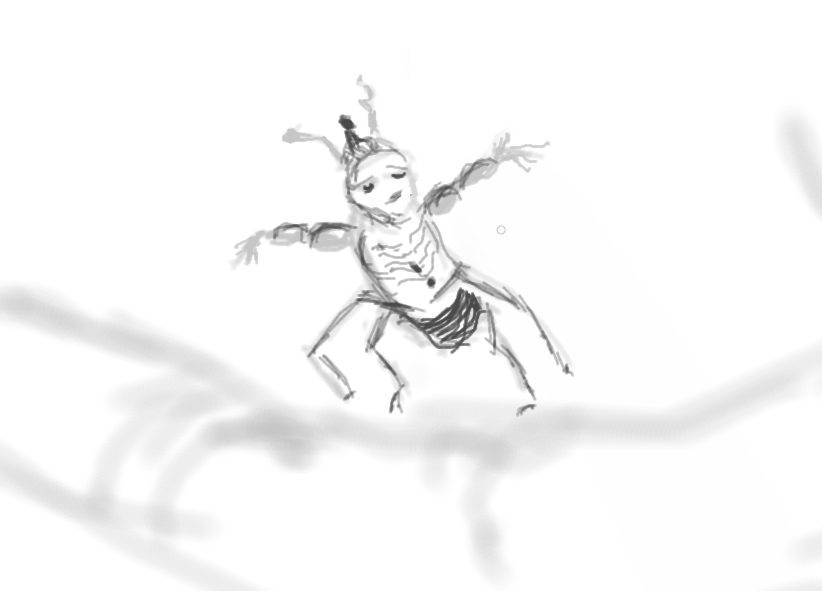
\includegraphics[width=0.6\textwidth]{images/paintings/jeff3b} }\\
		\caption{Dessins réalisés pendant les tests par \emph{Jean-François Brogniet}}
	\end{figure}
	\begin{figure}[h]
		\centering
		\subfloat[Étape 2: Familiarisation avec le programme]{
\includegraphics[width=0.5\textwidth]{images/paintings/jeanphi0} }
		\subfloat[Étape 3: Portrait au trait]{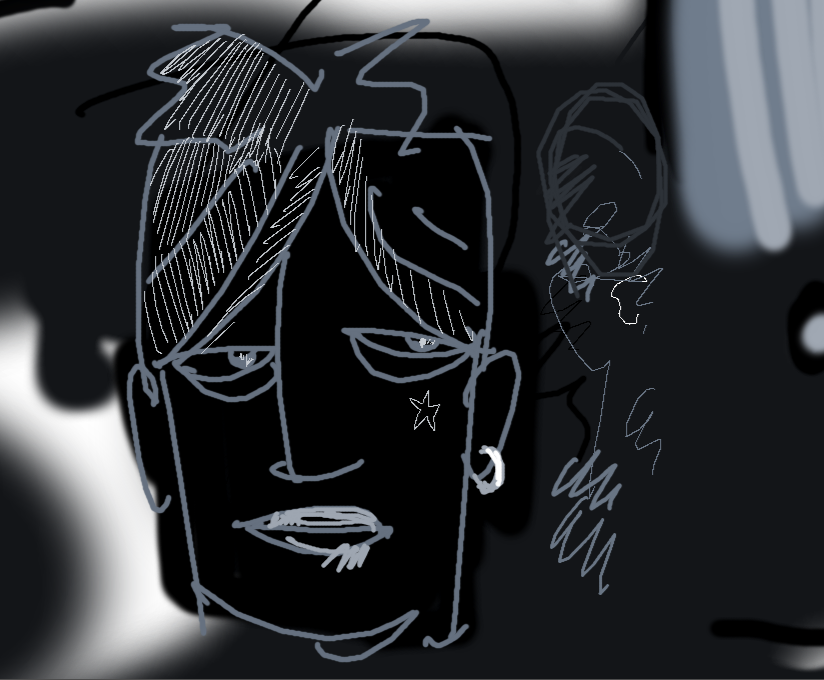
\includegraphics[width=0.5\textwidth]{images/paintings/jeanphi1} }\\
		\subfloat[Étape 4: Potrait couleur]{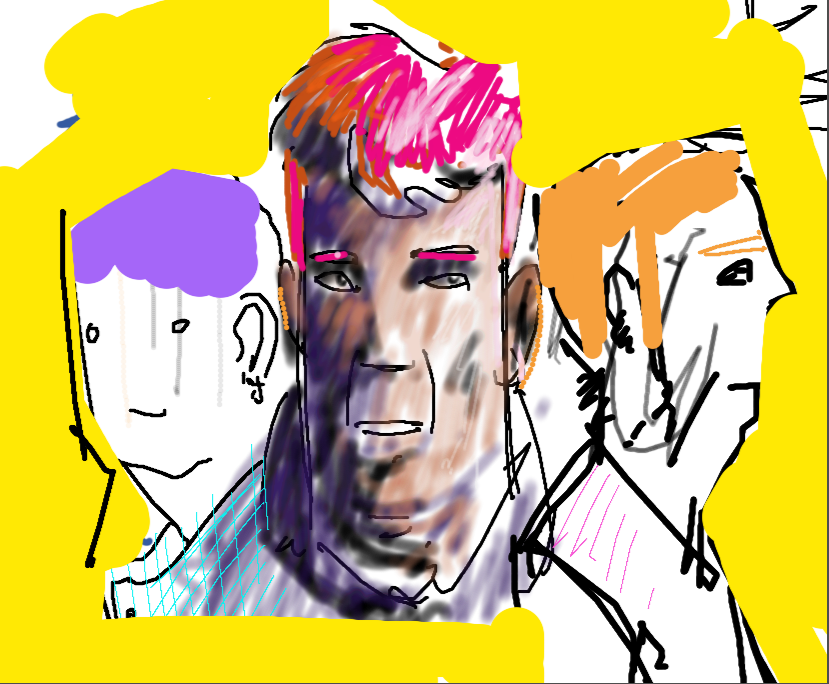
\includegraphics[width=0.5\textwidth]{images/paintings/jeanphi2} }
		\subfloat[Étape 5: Homme avec puce sur éléphant ]{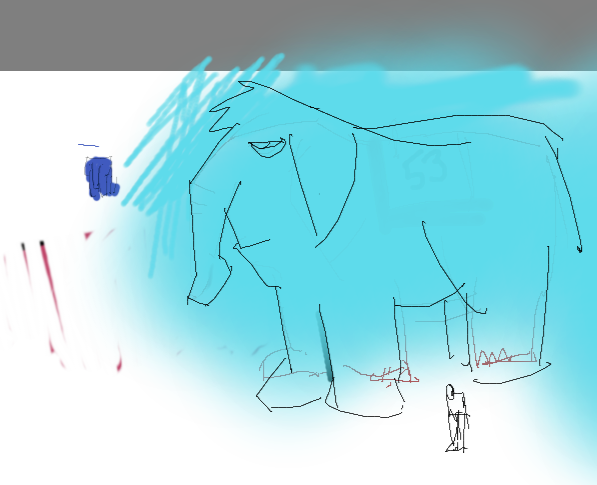
\includegraphics[width=0.5\textwidth]{images/paintings/jeanphi3} }\\
		\subfloat[Étape 5: Homme avec puce sur éléphant : Détail]{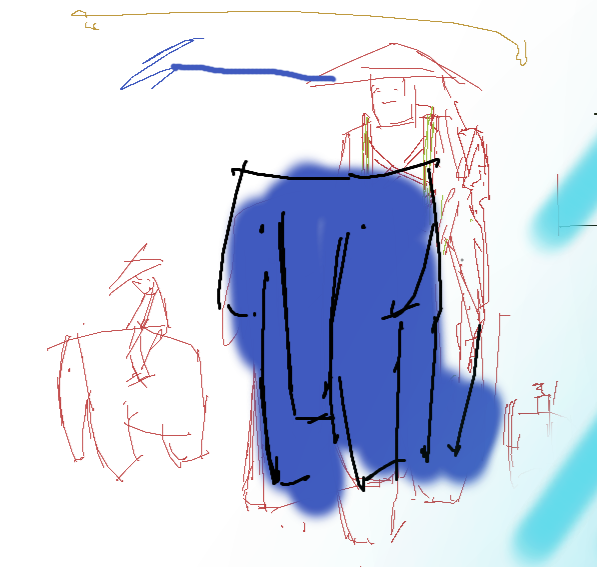
\includegraphics[width=0.6\textwidth]{images/paintings/jeanphi3b} }\\
		\caption{Dessins réalisés pendant les tests par \emph{Jean-Philippe Servais}}
	\end{figure}
	
	
	
